\newpage
\thispagestyle{empty}
\vspace*{\fill}
\begin{center}
    \large Parte III \\
    \vspace{0.5cm}           
    \LARGE \textbf{FUNDAMENTOS INFORMÁTICOS}
\end{center}
\vspace*{\fill}
\newpage


\chapter{Proyecto GEO (Gene Expression Omnibus)}

% esto ha salido de geo1, geo2, geo3
La información recogida en este capítulo dedicado a la base de datos \textit{GEO} ha sido extraída principalmente de las fuentes bibliográficas 
\cite{geo-1,geo-2,geo-3,geo-4,geo-overview}. \newline

\textit{Gene Expression Omnibus} (GEO) es una base de datos pública e internacional gestionada por el Centro Nacional de Información 
Biotecnológica (NCBI) de la Biblioteca Nacional de Medicina (NLM) de EE.UU.
Está diseñada para almacenar y distribuir de manera libre conjuntos de datos relacionados con la expresión génica y otros estudios 
genómicos funcionales. Acepta tanto datos crudos como procesados, siempre con una descripción detallada del 
diseño experimental, las características de las muestras y las metodologías utilizadas en los estudios de genómica de alto rendimiento. \newline

Fue lanzada en el año 2000 debido al rápido crecimiento de los datos de expresión génica generados por tecnologías como los microarrays y la secuenciación 
de ADN. GEO ofrece una estructura abierta y flexible, que permite enviar, almacenar y acceder a conjuntos de datos muy variados, procedentes de 
técnicas como RNA-seq, single-cell RNA-seq (scRNA-seq), arrays de proteínas o tejidos, RT-PCR, estudios de metilación del genoma, análisis de 
variaciones en el número de copias (CNV) y más. Aunque aproximadamente el 90\% de los datos en GEO corresponden a estudios de expresión génica, 
su alcance se ha expandido con el tiempo. Actualmente, recibe datos de alrededor de 72 países, consolidándose como un recurso global, gratuito 
y de acceso público. \newline

Aunque no tiene como objetivo reemplazar bases de datos internas especializadas en expresión génica, GEO complementa estas fuentes actuando como 
un repositorio terciario\footnote[1]{Un repositorio terciario se refiere a un sistema que integra y organiza datos de diversas 
fuentes primarias y secundarias, sirviendo como un centro de distribución más amplio y accesible.} y centralizado. Su función principal es ofrecer una plataforma 
donde se difunden datos provenientes de múltiples estudios y fuentes, facilitando el acceso a información crucial para la investigación. Ofrece herramientas 
para la consulta, visualización y análisis de estos datos directamente desde su página web, lo que hace que sea fácil de usar incluso para investigadores 
sin experiencia en bioinformática o software especializado.\newline

Además, GEO sigue las normas establecidas por la \textit{Functional Genomics Data Society}, adhiriéndose a las directrices MIAME (\textit{Minimum Information About a Microarray Experiment}) 
y MINSEQE (\textit{Minimum Information about a high-throughput SEQuencing Experiment}), lo que asegura que los datos sean interpretables y reproducibles 
por la comunidad científica. Estas directrices definen los requisitos mínimos de información que debe acompañar a cada experimento, permitiendo 
su correcta interpretación, reutilización y comparación con otros estudios. \newline

En lo que sigue, iremos detallando los tres objetivos principales que persigue GEO y que son:

\begin{itemize}
    \item[1.] Proporcionar una base de datos robusta y verátil para almacenar de manera eficiente datos genómicos funcionales de alto rendimiento
    (véase Organizacón de los datos).
    \item[2.] Ofrecer prodemientos y formatos de envío sencillos que permitan a la comunidad científica depositar datos completos y bien anotados
    (véase Envío de datos).
    \item[3.] Facilitar mecanismos intuitivos que permitan a los usuarios consultar, localizar, revisar y descargar estudios y perfiles de expresión génica
    de interés (véase Navegación, descarga y consulta).
\end{itemize}


\section{Organización de los datos}

% esto ha salido del overview de GEO y de mi cabeza

La base de datos GEO almacena una amplia varidad de experimentos genómicos a gran escala, los cuales generan datos en muchos formatos, tipos de archivos
y contenido. Esto presenta un gran desafío en cuanto a manejo y consulta de la información. \newline

Es por ello por lo que ha sido diseñada con una estructura que permite adaptarse a esta diversidad de datos. Cabe señalar que los datos que vienen en tablas
no se almacenan de forma complementamente estructurada dentro de la base de datos central, sino que se guardan como tablas de texto plano, delimitadas por
tabulaciones, sin límites en cantidad de filas y columnas. \newline

Los registros que hay almacenados en GEO, todos ellos proporcionados por los investigadores (\textit{submitters}) se organizan de la siguiente forma:

\begin{itemize}
    \item \textit{Platforms: } son registros compuestos por:
    \begin{itemize}
        \item Una descripción general del array o del secuenciador.
        \item En el caso de las basadas en arrays,incluye además una tabla de datos que define la plantilla del array.
    \end{itemize} 

        Cada registro Platform recibe un número de acceso único y estable en GEO, con el prefijo \textit{GPLxxx} (por ejemplo, GPL570). \newline

        Puede estar referenciada por muchas muestras (Samples), las cuales pueden haber sido enviadas por múltiples remitentes (investigadores).

    \item \textit{Samples: } una muestra describe:
    \begin{itemize}
        \item Las condiciones bajo las cuales se manejó una muestra individual.
        \item Las manipulaciones a las que fue sometida.
        \item Un archivo original de datos en crudo o archivo de datos de secuenciación, procesados.
    \end{itemize}
    Al igual que antes, cada muestra tiene un Id asociado que comienza por \textit{GSMxxx}. \newline

    Una muestra debe referenciar a una y solo una Platform, que debe estar previamente definida, pero puede estar incluida en múltiples Series.
    
    \item \textit{Series: } un registro en serie:
    \begin{itemize}
        \item Vincula un grupo de muestras relacionadas (Samples).
        \item Sirve como punto central y descriptivo del estudio completo, ofreciendo una descripción en texto del experimento en su conjunto.
        \item Incluye un archivo comprimido (.tar) que contiene los archivos originales de datos en crudo o los archivos de datos de secuenciación
        procesados.
    \end{itemize}

    Cada serie recibe un identificador único que empieza por \textit{GSExxx}.
\end{itemize}

Como la estructura de la base de datos se organiza en torno a entidades bien definidas, como Platform, Sample y Serie, que poseen atributos específicos
y mantienen relaciones entre sí con cardinalidades reconocibles, es lógico pensar que el diseño conceptual de GEO está basado en un modelo entidad-relación
y, por ende, el lógico basado en el modelo relacional, que se obtiene a partir del conceptual mediante paso a tablas. \newline

Cabe señalar que los archivos de datos en crudo que acompañan a los registros se almacenan en un servidor FTP\footnote{FTP (\textit{FIle Transfer Protocol}) 
es un servicio utilizado para el envío y obtención de archivos entre dos equipos remotos \cite{ftp}.} y están enlazados desde cada entrada. \newline

% referencia FTP: https://blog.infranetworking.com/servidor-ftp/ 

En base a toda esta información acerca de las entidades involucradas y sus relaciones, podemos construir un posible diagrama E/R para esta base de datos:

\begin{figure}[h]
    \centering
    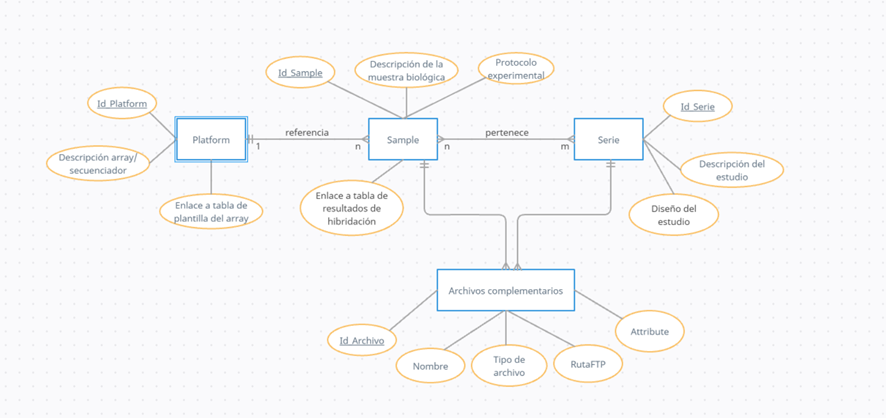
\includegraphics[width=1\textwidth]{../img/diagramaER.png}
    \caption{Diagrama Entidad-Relación (Fuente: elaboración propia).}
\end{figure}


% a lo mejor esto lo pongo en una sección a parte. Tendría que cambiar la introducción.
% esto ha salido del overview de GEO y de geo3.pdf

Por otra parte, los datos de \textit{Platform}, \textit{Sample} y \textit{Series} que envían los investigadores a GEO son bastante diversos en cuanto a formato, 
contenido y nivel de detalle con el que se describen los experimentos. Sin embargo, a pesar de estas diferencias, todas las presentaciones de estudios de expresión 
génica basados en arrays comparten una serie de elementos comunes:

\begin{itemize}
\item Información para identificar la secuencia de cada elemento presente en la \textit{Platform}. Es decir, cada sonda o fragmento de secuencia está asociado a 
una secuencia de nucleótidos específica, lo que permite localizarla de forma única y vincularla a un gen o región concreta del genoma.
\item Mediciones de expresión normalizadas incluidas en las tablas de \textit{Sample}.
\item Una descripción textual que recoge de dónde procede la muestra biológica y cuál es el objetivo del estudio.
\end{itemize}

Para organizar toda esta información y facilitar su consulta y análisis, se lleva a cabo un proceso que combina extracción automatizada de datos con una revisión 
manual, conocida como \textit{curación de datos}\footnote{La curación manual consiste en una revisión realizada por personal especializado que garantiza la calidad, 
consistencia y coherencia de los datos recopilados, corrigiendo posibles errores y asegurando que se ajustan a los estándares establecidos \cite{curacion-datos}.}. Gracias a este procedimiento, 
los datos enviados por los investigadores se reorganizan en registros más estructurados y accesibles denominados \textit{DataSets}. \newline

Un \textit{DataSet} agrupa un conjunto de muestras biológicas que son comparables entre sí desde un punto de vista biológico y estadístico, y que pertenecen a una 
misma \textit{Platform}. Esto significa que todas comparten el mismo conjunto de sondas o elementos en el array, y que las mediciones de expresión se han procesado 
aplicando criterios homogéneos de normalización y ajuste de fondo. De esta forma, se asegura que los valores se puedan comparar de forma adecuada. \newline

Además, a partir de estos \textit{DataSets} se generan los denominados \textit{Profiles}. Un \textit{Profile} consiste en las mediciones de expresión de un gen concreto 
a lo largo de todas las muestras incluidas en un \textit{DataSet}. Estos perfiles permiten estudiar cómo varía la expresión de un gen específico en diferentes condiciones 
experimentales o tipos de muestra, y se pueden consultar mediante la herramienta \textit{GEO Profiles}, que ofrece opciones de búsqueda y visualización específicas para 
este tipo de datos. Todos ellos se indexan en la base de datos \textit{Entrez GEO Profiles}. \newline

Es importante señalar que no todos los registros \textit{Series} que se envían a GEO acaban formando parte de un \textit{DataSet}. Este trabajo de selección y reorganización 
lo realiza el personal encargado de la curación y mantenimiento de la base de datos, que se encarga de elegir qué estudios reúnen las condiciones necesarias para integrarse 
en un \textit{DataSet}. Además, los \textit{DataSets} y \textit{Profiles} son la base para muchas de las herramientas de visualización y análisis que ofrece GEO, como los 
gráficos de perfiles de expresión génica o los clústeres de agrupación de muestras. Por último, cada \textit{DataSet} recibe un identificador único y estable con el prefijo 
\textit{GDS}, y se pueden consultar desde la interfaz \textit{Entrez GEO DataSets}.

\begin{figure}[h]
    \centering
    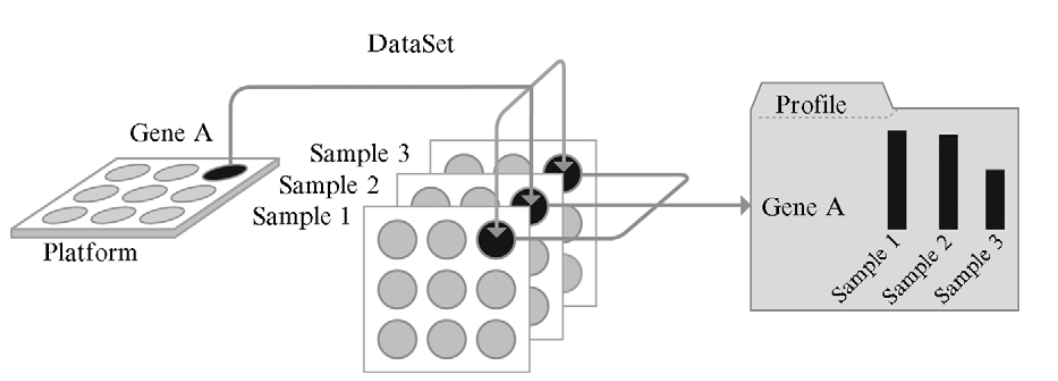
\includegraphics[width=1\textwidth]{../img/geo-datasets.png}
    \caption{Relación entre Platforms, Samples, DataSets y Profiles (Fuente: \cite{geo-4}).}  % geo-4.pdf
\end{figure}

% referencia curación manual:  https://es.wikipedia.org/wiki/Curaci%C3%B3n_de_datos

\section{Envío de datos}

% esto lo estoy viendo de geo4.pdf

Como se adelantó en la introducción, la base de datos GEO se adhiere a las reglas establecidas en MIAME y, por consiguiente, el envío de los procedimientos promueven
su cumplimiento. Sin embargo, es el propio investigador el que tiene la responsabiilidad, en última instancia, de asegurar que los datos estén suficientemente anotados y
que se cumple la normativa para investigación con sujetos humanos. A continuación se va a hacer un desglose de los pasos de los que se compone el flujo de datos que siguen 
los investigadores al enviar datos a GEO:

\begin{itemize}
    \item[1.] \textit{Inicio del depósito de datos:} Los investigadores envían sus datos a GEO antes de enviar su manuscrito a una revista. Esto lo hacen a través de su cuenta en 
    de MyNCBI.
    \item[2.] \textit{Formatos de envío:} GEO permite varios formatos de envío, como hojas de cálculo o XML, según las instrucciones de envío.
    \item[3.] \textit{Validación y curación:} Los envíos pasan primero porr una validación sintáctica automática. Luego, un curador de GEO revisa que los datos estén bien organizados
    y contengan suficente información. Si hay algún problema, el curador colabora con los autors hasta resolverlos.
    \item[4.] \textit{Asignación de identificadores:} Cuando todo está correcto, se asignan números de acceso estables que se pueden citar en el manuscrito.
    \item[5.] \textit{Privacidad previa a la publicación:} Los datos se mantienen privados hasta que el artículo es publicado. Durante ese tiempo, los autores pueden generar una URL
    que dé acceso conficencial a editores y revisores.
    \item[6.] \textit{Disponibilidad pública e indexación:} Tras su publicación, los datos de Platform, Sample y Serie se indexan en la base de datos \textit{Entrez GEO DataSets}, donde
    los usuarios pueden consultar y descargar los datos, o realizar un análisis de expresión génica mediante la herramienta de comparación \textit{GEO2R}.
    \item[7.] \textit{Interoperabilidad con otras bases de datos:} Alguna partes del envío se transiferen a otras bases de datos como \textit{SRA} (para secuencias) o \textit{BioProject}
    (para descripciones de estudios), con enlaces recíprocos hacia GEO.
    \item[8.] \textit{Curación mensual adicional:} Cada mes, algunas Series se seleccionan para una curación más profunda, creando \textit{GEO DataSets} y \textit{GEO Profiles}, derivados 
    de estos.
    
\end{itemize}

\section{Navegación, descarga y consulta}


\subsection{Navegación}
% https://www.ncbi.nlm.nih.gov/geo/browse/

El navegador de repositorios GEO cuenta con pestañas que contienen tablas donde se listan los registros de Series, Samples, Platforms y DataSets. Las tablas incluyen información que se 
puede buscar y filtrar, así como enlaces a registros relacionados y descargas de archivos complementarios. Estas tablas se pueden exportar e incluyen información adicional que no se muestra
en el navegador, como identificadores de \textit{PubMed} y accesiones relacionadas en SRA.

\begin{figure}[h]
    \centering
    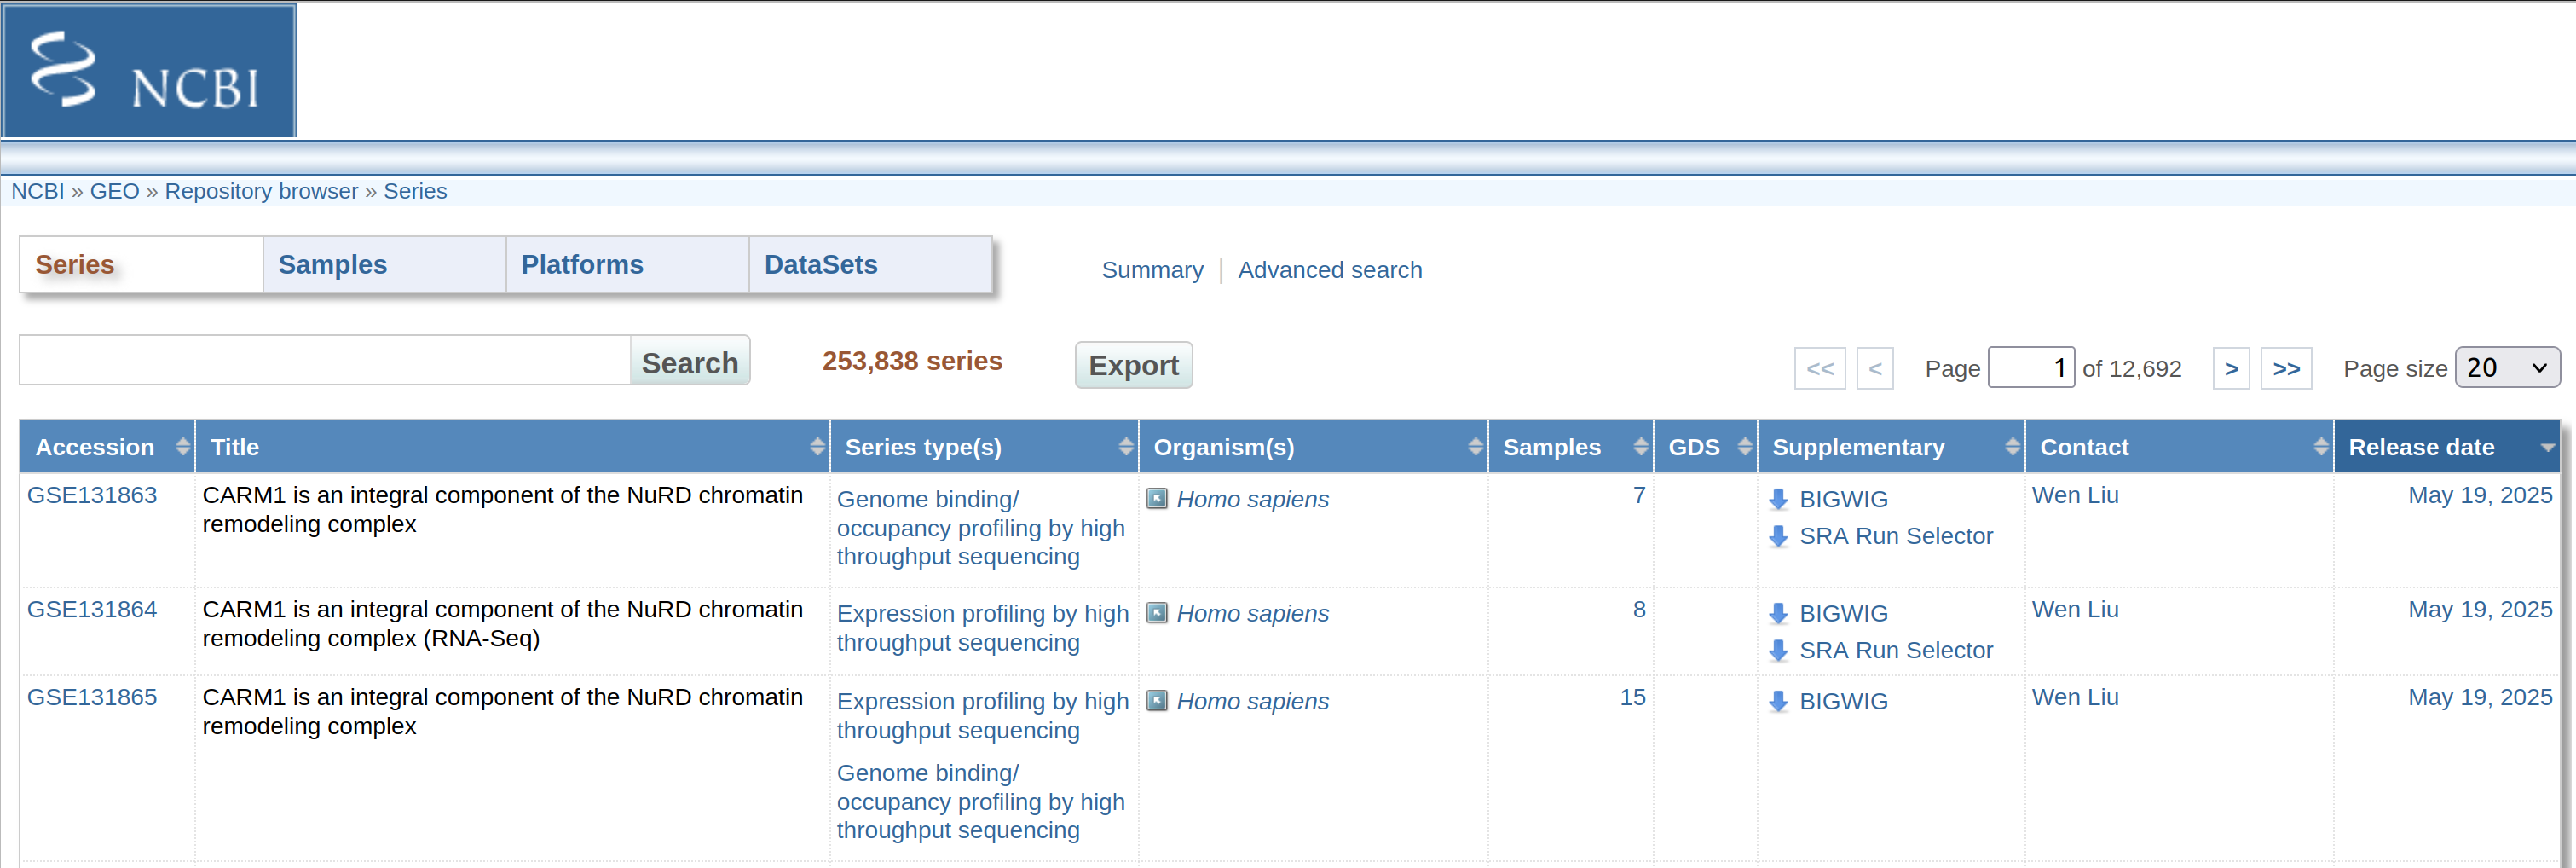
\includegraphics[width=1\textwidth]{../img/geo-browser.png}
    \caption{Navegador GEO (Fuente: \cite{geo-browse}).}
\end{figure}

\subsection{Descarga de datos}

Todos los datos almacenados en GEO pueden descargarse en una gran variedad de formatos usando varios mecanismos que se presentan a continuación.

Para descargar registros GEO originales podemos hacerlo de cualquiera de las siguientes formas:

\begin{itemize}
    \item \textit{Enlaces a registros de Series:} Al pie de cada registro Serie de GEO, figuran enlaces a descargas de familias de experimentos en diversos formatos y archivos complementarios.
    Estos archivos están comprimidos con gzip (extension .gz o .tgz). Para descomprimir y leer estos archivos, se ha de utilizar la herramienta \textit{WinZip} o \textit{7-Zip}.
    \item \textit{Descarga FTP:} Todos los registros GEO y los archivos de datos en crudo pueden descargarse gratuitamente desde el sitio FTP de GEO. Sin embargo, GEO contiene a día de hoy tal
    cantidad de envíos que ya no se puede acceder a algunos directorios principales mediante navegadores web debido a errores de latencia. En tales casos, es necesario pasar por alto el directorio 
    principal e ir directamente al directorio de destino. Por ejemplo, para la serie \textit{GSE1000}:

    \[
        ftp://ftp.ncbi.nlm.nih.gov/geo/series/GSE1nnn/GSE1000/matrix/ 
    \]
    
    La mayoría de los archivos del servidor FTP están comprimidos con gzip (extensión .gz y .tgz). Para descomprimirlos y leerlos, si se usa Windows, se puede hacer con WinZip o 7-Zip. Si se dispone 
    de UNIX, se deberán de seguir los comandos tar y gunzip para extraer los archivos, por ejemplo: \newline

    \begin{lstlisting}[language=bash, backgroundcolor=\color{lightgray}, basicstyle=\ttfamily, keywordstyle=\color{blue}, numbers=none]
    $ tar -xf GSExxxx_RAW.tar
    $ gunzip *gz \end{lstlisting}
        
    \item  \textit{Barra de visualización por identificadores (\textit{Accessions}):} Se encuentra en la parte superior de cada registro GEO y puede utilizarse para descargar o visualizar registros completos o parciales,
    Platforms, Samples y Series relacionados. La función \textit{Scope} (el alcance) permite visualizar un único número de acceso (\textit{Self}), cualquiera (\textit{Platform, Sample o Serie}),
    o todos (\textit{Family}) los registros relacionados con el acceso especificado (el identificador que hayamos puesto). \textit{Amount} determina la cantiad de datos mostrados con opciones que incluyen 
    sólo metadatos (\textit{Brief}), metadatos y las 20 primeras filas de la tabla de datos (\textit{Quick}), sólo tabla de datos (\textit{Data}) o registros completos de metadatos/tabla de datos (\textit{Full}). 
    \textit{Format} controla si los registros se muestran en formato HTML, SOFT (texto sin formato) o MINiML (XML).

    \begin{figure}[h]
        \centering
        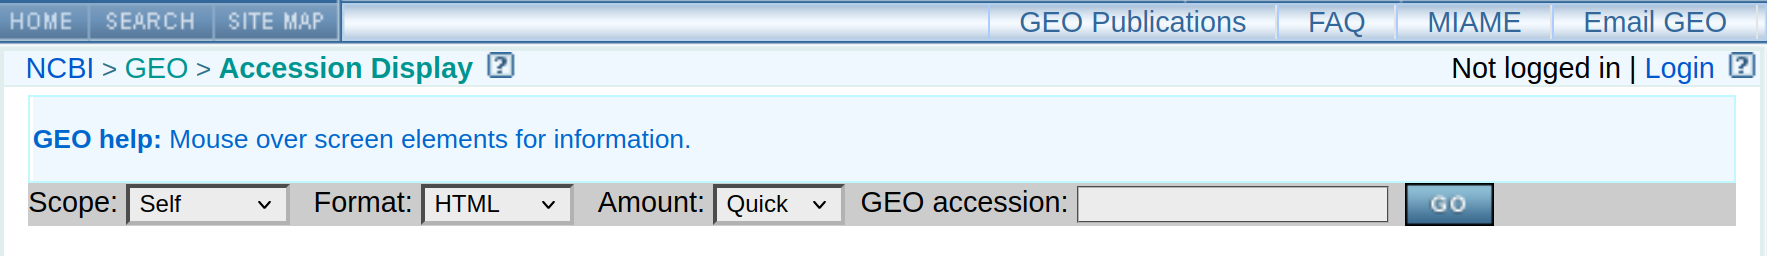
\includegraphics[width=1\textwidth]{../img/geo-displayBar.png}
        \caption{Barra de navegación de accesiones (Fuente: \cite{display-bar}).}  % https://www.ncbi.nlm.nih.gov/geo/query/acc.cgi
    \end{figure}
    \item \textit{Construcción de una URL:} Una forma alternativa de usar la barra de visualización de accesos anteriormente descrita, es construir una URL para devolver los datos que nos interesen. Las URLs 
    tienen el siguiente formato: 

    
    \url{https://www.ncbi.nlm.nih.gov/geo/query/acc.cgi?acc=gpl96&targ=self&view=brief&form=text}


    Esta URL, bajo el esquema http y la autoridad \textit{www.ncbi.nlm.nih.gov}, accederá a \textit{acc.cgi} a través de la ruta \textit{geo/query/acc.cgi} y realizará una consulta para devolver un fichero de 
    texto que contiene una breve vista de la accesión \textit{GPL96}. \newline  % partes de una URI tema 1 PW

    Los posibles valores para las componentes de la consulta son:

    \begin{itemize}
        \item \textit{acc} = un identificador GEO válido, según el formato \textit{glpxxx, gsmxxx} o \textit{gsexxx}.
        \item \textit{targ} = \textit{self, gsm, gpl, gse} o \textit{all}.
        \item \textit{view} = \textit{brief, quick, data} o \textit{full}.
        \item \textit{form} = \textit{text, html} o \textit{xml}.
    \end{itemize}

    \item \textit{Descargas de consultas en Entrez GEO DataSets:} Todos los registros originales pueden buscarse y descargarse a través de la interfaz \textit{Entrez GEO DataSets.} Los resultados pueden exportarse
    configurando la barra de herramientes de la parte superior de la página como \textit{'Enviar a: Archivo'}.
        
\end{itemize}


Para descargar \textit{DataSets} y \textit{Profiles} curados, podemos usar:

\begin{itemize}
    \item \textit{Enlaces en DataSets}: Los enlaces a los archivos \textit{SOFT} de \textit{DataSet} están disponibles en el botón <<download>> de cada registro de \textit{DataSet}. Estos archivos están comprimidos
    con gzip.
    \item \textit{Descarga FTP:} Todos los registros \textit{GEO DataSet} están disponibles, como hemos dicho antes, en el servidor FTP de GEO.
    \item \textit{Valores de Perfil:} Para descargar datos de perfil, usamos el botón \textit{Download profile data} situado en la parte superior de las páginas de recuperación de 
    \textit{Entrez GEO Profiles} para descargar los valores de expresión de los genes encontrados en la consulta.
    \item \textit{Descargas de consultas a Entrez GEO DataSets y Entrez GEO Profiles:} Es posible exportar resúmenes de documentos de \textit{Entrez GEO DataSets} y \textit{Entrez GEO Profiles} configurando la barra
    de herramientas de la cabecera de la página como \textit{'Enviar a: Archivo'}.
\end{itemize}

\subsection{Consulta de datos}

% se ha sacado de geo3.pdf 

NCBI dispone de un potente sistema de búsqueda y recuperación llamado \textit{Entrez}, que permite consultar el contenido de su red de bases de datos integradas. Los datos de GEO están disponibles en dos bases de
datos independientes a las que ya hemos hecho referencia en numerosas ocasiones: \textit{Entrez GEO DataSets} y \textit{Entrez GEO Profiles}. \newline

El flujo de trabajo habitual consiste en que el usuario primero identifique estudios de interés mediante la búsqueda en \textit{Entrez GEO DataSets}, y posteriormente utilice \textit{GEO2R} o \textit{GEO Profiles} para
localizar genes específicos o patrones de expresión génica dentro de ese estudio. También es posible consultar directamente \textit{Entrez GEO Profiles}. \newline

Además, \textit{Entrez} genera numerosos enlaces que conectan datos relacionados: enlaces entre bases de datos que vinculan GEO con otros recursos de NCBI como \textit{PubMed}, \textit{GenBank} o \textit{Gene}; y enlaces
dentro de la propia base de datos, que conectan genes relacionados por patrón de expresión, posición cromosómica o secuencia. \newline

Ambas bases de datos permiten refinar búsquedas mediante filtros por campos específicos, búsqueda por facetas, que sería la forma más sencilla de consulta, y consultas avanzadas combinadas. \newline

Veamos cómo se puede consultar la base de datos \textit{Entrez GEO DataSets} mediante consultas avanzadas. Como ya se ha mencionado anteriormente, esta base de datos almacena las descripciones originales de los registros de Platform, Sample y Series
aportados por los autores, así como los \textit{DataSets} curados. Puede buscarse utlizando distintos atributos como palabras clave, organismo, tipo de estudio o autores. 

\begin{figure}[h]
    \centering
    
\includegraphics[width=1\textwidth]{../img/geo-datasets-browser.png}
    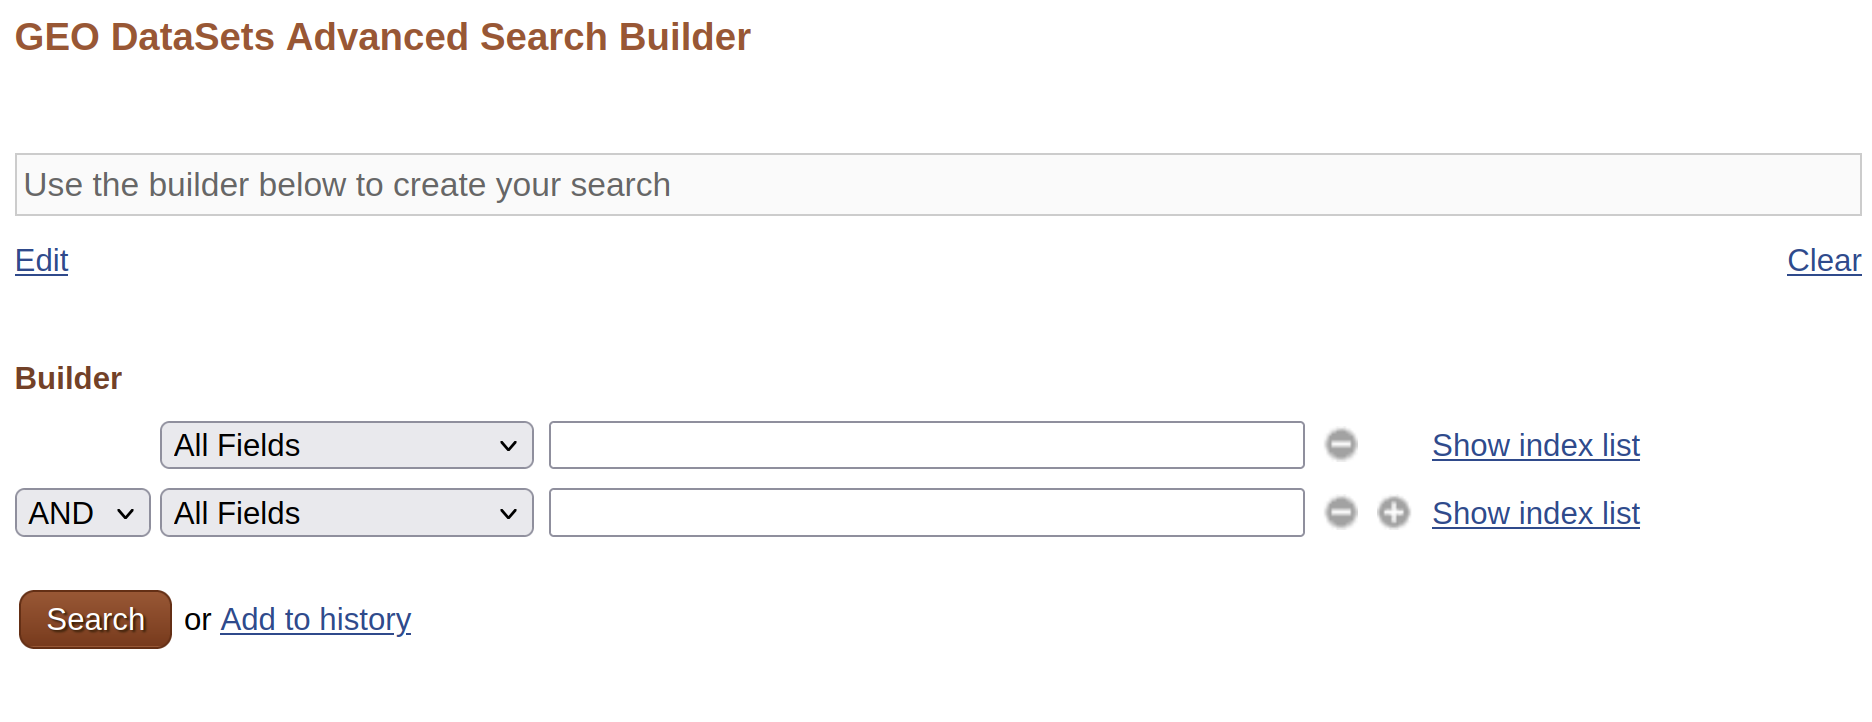
\includegraphics[width=1\textwidth]{../img/geo-adv-queryDataset.png}
    \caption{Construcción de consulta avanzada en \textit{Entrez GEO DataSets} (Fuente: \cite{geo-advanced}).}  % https://www.ncbi.nlm.nih.gov/gds/advanced
\end{figure}

Algunos ejemplos de consultas serían:

\begin{itemize}
    \item Recuperar estudios que investigan el efecto del tabaco o la dieta en mamíferos no humanos:
    \begin{lstlisting}[basicstyle=\ttfamily\small, backgroundcolor=\color{lightgray}, numbers=none, aboveskip=0pt, belowskip=0pt]
(smok* OR diet) AND (mammals[organism] NOT human[organism])\end{lstlisting}

    \item Buscar estudios que analicen expresión génica mediante secuenciación de nueva generación:
    \begin{lstlisting}[basicstyle=\ttfamily\small, backgroundcolor=\color{lightgray}, numbers=none, aboveskip=0pt, belowskip=0pt]
"expression profiling by high throughput sequencing"[DataSet Type]\end{lstlisting}

    \item Recuperar envíos que incluyan archivos Affymetrix CEL:
    \begin{lstlisting}[basicstyle=\ttfamily\small, backgroundcolor=\color{lightgray}, numbers=none, aboveskip=0pt, belowskip=0pt]
cel[Supplementary Files]\end{lstlisting}

    \item Localizar DataSets curados que incluyan 'edad' como variable experimental:
    \begin{lstlisting}[basicstyle=\ttfamily\small, backgroundcolor=\color{lightgray}, numbers=none, aboveskip=0pt, belowskip=0pt]
age[Subset Variable Type]\end{lstlisting}

    \item Consultar estudios que contengan entre 100 y 500 muestras:
    \begin{lstlisting}[basicstyle=\ttfamily\small, backgroundcolor=\color{lightgray}, numbers=none, aboveskip=0pt, belowskip=0pt]
100:500[Number of Samples]\end{lstlisting}

    \item Buscar estudios en los que aparezca ‘Smith, A.’ como autor:
    \begin{lstlisting}[basicstyle=\ttfamily\small, backgroundcolor=\color{lightgray}, numbers=none, aboveskip=0pt, belowskip=0pt]
smith a[Author]\end{lstlisting}

\end{itemize}

Por su parte, como ya se mencionó anteriormente, la base de datos \textit{Entrez GEO Profiles}, almacena perfiles de expresión génica derivados de \textit{DataSets} curados de GEO.
Cada perfil se muestra como un gŕafico que representa el nivel de expresión de un gen a lo largo de todas las muestras de un \textit{DataSet}. En la parte inferior del bráfico hay unas
barras que indican el contexto experimental, lo que permite ver fácilmente si un gen está diferencialmente expresado en distintas condiciones. \newline

\begin{figure}[h]
    \centering
    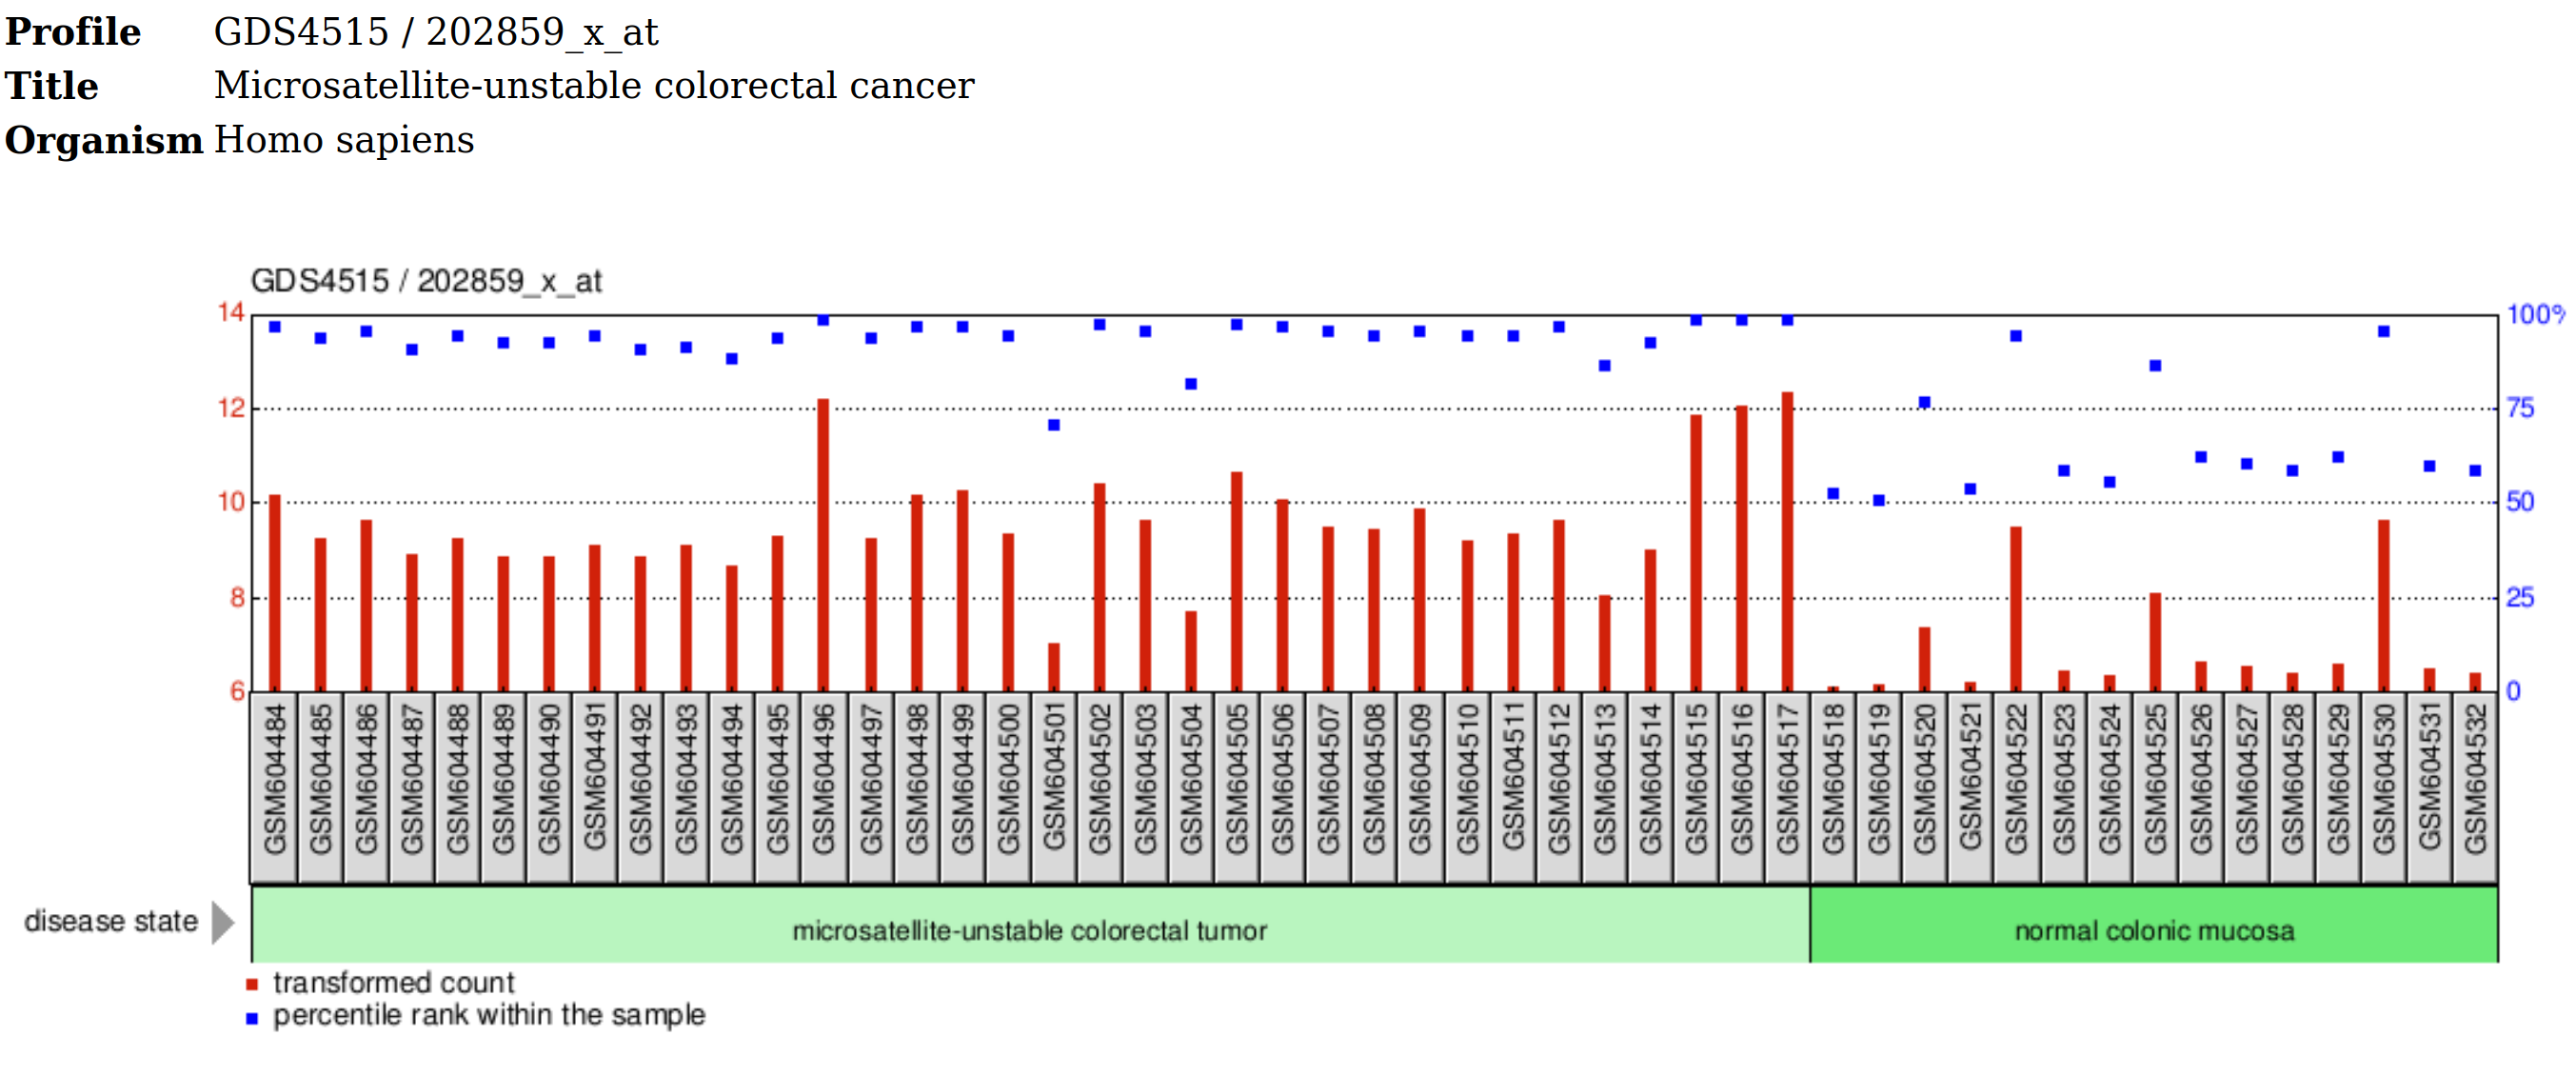
\includegraphics[width=1\textwidth]{../img/geo-profile.png}
    \caption{Ejemplo de perfil (Fuente: \cite{geo-profile}).}  % https://www.ncbi.nlm.nih.gov/geo/tools/profileGraph.cgi?ID=GDS4515:202859_x_at
\end{figure}

Se puede consultar usando diferentes atributos, como palabras clave, símbolos o nombres de genes, identificadores de \textit{GenBank} o perfiles que estén marcados como diferencialmente expresados.
Algunos ejemplos de consultas incluyen:

\begin{itemize}
    \item Recuperar todos los perfiles de expresión génica para CYP1A1:
    \begin{lstlisting}[basicstyle=\ttfamily\small, backgroundcolor=\color{lightgray}, numbers=none, aboveskip=0pt, belowskip=0pt]
CYP1A1[Gene Symbol]\end{lstlisting}

    \item Recuperar perfiles de expresión génica de CYP1A1 o ME1 en DataSets que investiguen los efectos del tabaco o la dieta:
    \begin{lstlisting}[basicstyle=\ttfamily\small, backgroundcolor=\color{lightgray}, numbers=none, aboveskip=0pt, belowskip=0pt]
(CYP1A1[Gene Symbol] OR ME1[Gene Symbol]) AND (smok* OR diet)\end{lstlisting}

    \item Recuperar perfiles para todas las quinasas en el DataSet con número de accesión GDS182:
    \begin{lstlisting}[basicstyle=\ttfamily\small, backgroundcolor=\color{lightgray}, numbers=none, aboveskip=0pt, belowskip=0pt]
kinase[Gene Description] AND GDS182\end{lstlisting}

    \item Recuperar perfiles para genes que tengan el término Gene Ontology (GO) ‘apoptosis’ en el DataSet con accesión GDS182:
    \begin{lstlisting}[basicstyle=\ttfamily\small, backgroundcolor=\color{lightgray}, numbers=none, aboveskip=0pt, belowskip=0pt]
apoptosis[Gene Ontology] AND GDS182\end{lstlisting}

    \item Recuperar perfiles de genes que se encuentren dentro del rango 10000:3000000 en el cromosoma 8 de ratón:
    \begin{lstlisting}[basicstyle=\ttfamily\small, backgroundcolor=\color{lightgray}, numbers=none, aboveskip=0pt, belowskip=0pt]
(8[Chromosome] AND 10000:3000000[Base Position]) AND mouse[organism]\end{lstlisting}

    \item Recuperar genes que muestran expresión diferencial en DataSets que examinan el efecto de un agente:
    \begin{lstlisting}[basicstyle=\ttfamily\small, backgroundcolor=\color{lightgray}, numbers=none, aboveskip=0pt, belowskip=0pt]
agent[Flag Information] AND "value subset effect"[Flag Type]\end{lstlisting}
\end{itemize}


Tras haber explorado en detalle la base de datos GEO, la organización de los datos y las herramientas de descarga y consulta, en la siguiente sección nos centraremos en \textit{Bioconductor}, un conjunto de paquetes de software en R 
diseñado para el análisis e interpretación de datos genómicos. Veremos cómo Bioconductor permite aprovechar al máximo la información obtenida de GEO mediante potentes técnicas estadísticas y bioinformáticas.

\newpage

\chapter{Bioconductor}  % referencias: https://bioconductor.org/about/ https://bioinformatics.ccr.cancer.gov/docs/rintro/Lesson_8/, bioconductor-2.pdf, bioconductor-1.pdf

La información recogida en este capítulo ha sido extraída principalmente de las fuentes bibliográficas \cite{bioconductor-1,bioconductor-about,bioconductor-about2,bioconductor-2}. \newline

Bioconductor es un proyecto de código abierto y un repositorio de paquetes para R que se usa mucho en bioinformática y biología computacional. 
Básicamente, es una plataforma que ofrece muchas herramientas para analizar datos biológicos, especialmente en el campo de las ómicas. 
La idea principal del proyecto es crear y compartir software libre que ayude a realizar análisis de datos biológicos de forma rigurosa y reproducible.

\section{Objetivos del proyecto}

Desde que empezó en 2001, Bioconductor ha ido adaptándose a nuevas tecnologías, desde los microarrays hasta la transcriptómica espacial, que 
es una técnica más reciente. Sus objetivos son varios, pero entre los principales están:

\begin{itemize}
\item Dar acceso a métodos estadísticos y gráficos avanzados para analizar datos genómicos.
\item Facilitar la incorporación de metadatos biológicos en estos análisis.
\item Ofrecer una plataforma común que permita desarrollar software que sea fácil de ampliar, escalable y que funcione bien con otras herramientas.
\item Promover la creación de documentación clara y la reproducibilidad en los estudios.
\item Formar a investigadores para que puedan usar técnicas computacionales y estadísticas en el análisis de datos genómicos.
\end{itemize}

\section{Integración de R en Bioconductor}
Para conseguir esto, Bioconductor se apoya en R, que es un lenguaje interpretado y de alto nivel muy usado en estadística y ciencia de datos. R permite 
crear de forma rápida nuevas formas de analizar datos, tiene un sistema para empaquetar el software junto con la documentación y ofrece estructuras orientadas a 
objetos que ayudan a manejar la complejidad de los problemas en biología computacional. Además, da acceso a datos en línea y tiene herramientas para 
hacer simulaciones, modelado y visualizar resultados.

Bioconductor aprovecha todo esto y añade sus propias estructuras y métodos para trabajar con datos genómicos a gran escala, como secuenciación de ADN, 
ARN o microarrays. También facilita crear flujos de trabajo donde se combinan diferentes tipos de datos y métodos estadísticos, regresión, análisis de 
redes, aprendizaje automático y visualización.


\section{Paquetes}

Los paquetes de Bioconductor se dividen en cuatro grupos principales:

\begin{itemize}
\item \textit{Software:} algunos paquetes proporcionan las bases para almacenar y acceder a los datos, y otros ofrecen herramientas para analizar esos 
datos. Esta separación hace que sea más fácil reutilizar estructuras y probar distintas formas de análisis sin aprender cosas nuevas cada vez.
\item \textit{Datos de anotación:} contienen bases de datos con información genómica como identificadores de genes o rutas biológicas.
\item \textit{Datos experimentales:} son conjuntos de datos estándar que se usan para mostrar ejemplos en los que se aplican los paquetes.
\item \textit{Workflows:} son colecciones de documentos que explican cómo usar varios paquetes juntos para hacer un análisis completo, pero no tienen 
código nuevo.
\end{itemize}


\section{GEO y Bioconductor}

Dado que \textit{GEO} es una de las bases de datos públicas más completas y utilizadas para almacenar datos de expresión génica, resulta muy interesante
poder integrarla con \textit{Bioconductor}. Así, tendríamos una fuente bastante extensa de datos sobre los que aplicar todo el potencial de los paquetes 
que ofrece Bioconductor. Para hacer posible esta conexión se desarrolló el paquete \textit{GEOquery}, que actúa como puente entre ambos, facilitando la 
descarga, consulta y manipulación de los datos desde R y su uso dentro del ecosistema de Bioconductor.

\subsection{GEOquery}

El objetivo principal de \textit{GEOquery} es descargar y leer los archivos en formato SOFT que usa GEO, manteniendo toda la información de los registros 
originales. Lo bueno de \textit{GEOquery} es que hace muy fácil acceder a los datos de GEO desde R, ya que básicamente todo se puede hacer con un único comando:
\texttt{getGEO}. \newline

Por ejemplo, para descargar un dataset completo (en este caso, el \textit{GDS1}), primero se carga la librería:

\begin{verbatim}
    library(GEOquery)
\end{verbatim}

Luego se usa el comando:

\begin{verbatim}
    gds <- getGEO('GDS1')
\end{verbatim}

Esto descarga el archivo comprimido en una carpeta termporal, lo descomprime, lo interpreta y lo guarda en una variable de R llamada \texttt{gds}. Esa
variable contiene ya todos los datos de GDS1 organizados en una estructura de tipo \texttt{GDS} que se puede utilizar dentro de R y Bioconductor. También
se puede hacer lo mismo con una muestra individual, cambiando el identificador del dataset por el de la muestra (\textit{GSMxxx}).

\subsubsection{Estructuras de datos en GEOquery}

Una de las ventajas que tiene \textit{GEOquery} es que organiza la información descargada en estructuras de datos específicas para facilitar su manejo. Estas
estructuras se agrupan de la misma forma en la que GEO organiza sus datos:

\begin{itemize}
    \item \textit{GDS,GPL y GSM:} son las clases básicas. Cada una contiene una cabecera con metadatos (extraídos tal cual de GEO) y una tabla llamada 
    \textit{GEODataTable}. Esta tabla tiene dos partes: los nombres de las columnas y una tabla de datos 2D. Por ejemplo, para consultar los metadatos de una
    muestra:
    \begin{verbatim}
    Meta(gsm)[1:3]
    \end{verbatim}

    Y para ver parte de la tabla de datos:

    \begin{verbatim}
    Table(gsm)[1:3,c(2,6,7)]
    \end{verbatim}

    O las descripciones de las columnas:

    \begin{verbatim}
    Columns(gsm)[c(2,6,7),]
    \end{verbatim}

    La clase \texttt{GPL} funciona igual, pero en vez de datos de expresión contiene información sobre las características de los arrays. Por otro lado, \texttt{GDS} 
    incluye además anotaciones asociadas a cada muestra.

    \item \textbf{GSE:} es una clase compuesta que representa un conjunto de muestras (GSM) y plataformas (GPL). Tiene su propia sección de metadatos, pero en 
    lugar de una tabla de datos, contiene dos listas: una con objetos \texttt{GPL} y otra con objetos \texttt{GSM}. Gracias a los métodos de acceso y a las capacidades 
    de manipulación de datos de R, se pueden consultar y reorganizar estos datos de forma flexible para los análisis que se quieran hacer.
\end{itemize}

\subsubsection{Conversión a estructuras de Bioconductor}

Los datos de \textit{GEO} tienen una estructura parecida a la de objetos usados en otros paquetes de \textit{Bioconductor}, como \texttt{MAList}(de \texttt{limma}) o 
\texttt{ExpressionSet} (de \texttt{Biobase}). Por eso, existen funciones como \texttt{GDS2MA} y \texttt{GDS2eSet} que permiten convertir un objeto \texttt{GDS} a estos 
formatos. \newline

Por ejemplo, para pasar el objeto \texttt{gds} que descargamos antes a un \texttt{ExpressionSet}:

\begin{verbatim}
    eset <- GDS2eSet(gds, do.log2 = TRUE)
\end{verbatim}

Así se obtiene un \texttt{ExpressionSet} que contiene los datos de GEO junto con la información de las muestras, los datos transformados en logaritmo (si se especifica) 
y las anotaciones de las sondas de la plataforma asociada. \newline

Además, existen funciones parecidas para convertir a otros tipos de objetos de Bioconductor, lo que permite integrar estos datos directamente en los análisis de expresión 
génica, clasificación, visualización o análisis de redes que se hacen con otros paquetes del entorno. \newline

En resumen, \texttt{GEOquery} sirve de puente entre las herramientas de Bioconductor y los datos públicos disponibles en GEO. Este puente es el que usaremos para desarrollar
la aplicación con la que pondremos fin a este trabajo y cuyo diseño, desarrollo y documentación veremos en profundidad en el siguiente capítulo. \newline